\section{Case Study 1}

The pilot case study implements the movie ticket reservation system prototype described in the outline earlier, primarily using microservices communicating with REST APIs. Representational State Transfer implies that a client requesting a resource from any service, cues the server to transfer back the current state of the resource in a standardised representation. The system design and implementation details are elaborated below.

\subsection{Design and Implementation}

\begin{figure}[H]
  \centering
  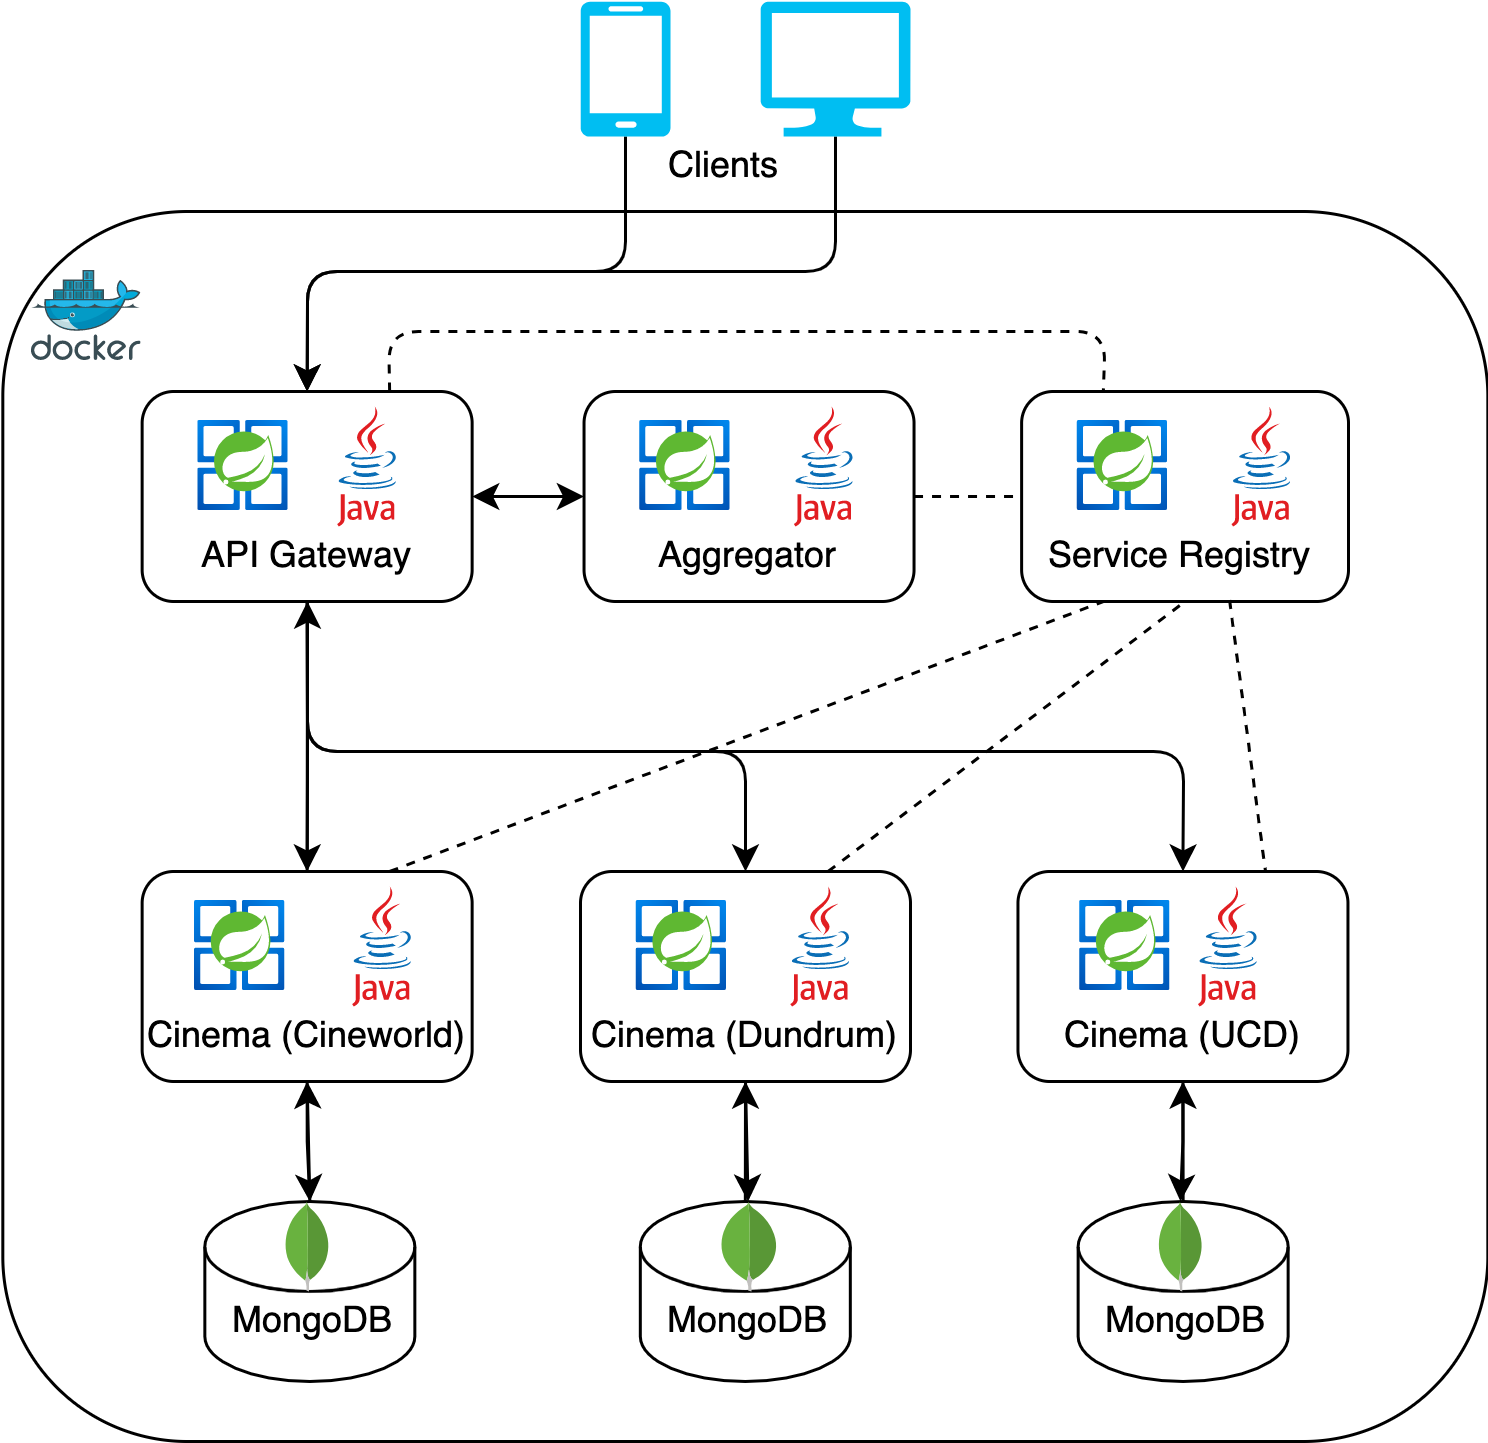
\includegraphics[width=0.6\linewidth]{./assets/diagrams/cs01-arch.png}
  \caption{System design for the first case study.}
  \label{fig:cs01-arch}
\end{figure}

The architecture diagram in Fig. \ref{fig:cs01-arch} depicts the organisation of the microservices involved: an API gateway service to act as an interface between clients and other services, and aggregator service to gather results, a central service registry, and three independent cinema services - Cineworld, Dundrum and UCD. The following microservice design patterns have been employed while developing this web application:

\subsubsection{API Gateway}

An \textit{API gateway} is one of the most fundamental and commonly used design patterns in microservice architecture. The \code{api-gateway-service} microservice offers an entry point for all clients, so that multiple services (e.g. cinemas) can be exposed, and gateway can route requests to other services as appropriate. In such situations, an API gateway relieves the clients from setting up and managing a separate endpoint for every service. It also aids the inter-service communication between microservices when required, for instance, the \code{aggregator-service} contacts the cinema services via the gateway again.

Without a gateway, any change (e.g. refactoring) in the service APIs would necessitate corresponding changes in the client code as well, which creates several development and management troubles. However, when a gateway is placed between clients and services, further consolidation or decomposition of a service would only require a simple routing change, instead of updating the client.

An added benefit of this pattern would be the ease of deployment of new versions of microservices, which can be done in parallel with existing versions, since API gateway routing would provide control over endpoints presented to clients, and flexibility over feature release strategies.

A minor variation of the API gateway pattern is called \textit{backends for frontends (BFF)}, where a separate gateway handles request routing for different kinds of clients, such as web applications, mobile applications and third part applications (e.g. IoT devices). API endpoint management in appropriate gateway services is a more focussed approach to handling routing logic for different kinds of user interfaces, with their own set of pre-requisites.

Despite its popularity and usefulness, the API gateway pattern brings with it a few issues that should be taken into consideration. For instance, it could become a bottleneck or single point of failure, if resiliency and fault tolerance measures are not put in place. Performance testing methods such as load testing should be explored to prevent failure scenarios.

In this case study, the \code{api-gateway-service} uses the Spring Cloud \footnote{\url{https://spring.io/projects/spring-cloud}} project to introduce a gateway \footnote{\url{https://spring.io/projects/spring-cloud-gateway}} in the application. The gateway is configured using the module's \code{application.yml} resource file, which Spring Boot \footnote{\url{https://spring.io/projects/spring-boot}} can access to set up all the routing logic supported by the application. From a performance perspective, an API gateway provides several benefits, such as options to set up request authentication, rate-limiting to prevent service over-use and DDoS attacks, monitoring and analytics endpoints (using Spring Boot Actuator), reducing latency by serving cached responses, as well as load balancing. A very simple gateway configuration example is shown below. The \code{lb://} prefix in \code{uri:} makes use of Spring Cloud Gateway's built-in load balancer, to provide round robin client-side load balancing features during calls to other microservices. A 503 Service Unavailable Error is returned when a service cannot be found, which is more appropriate than a basic Java exception stack trace shown when using \code{http://} or \code{https://} prefixes instead.

\begin{lstlisting}[caption=Sample Spring Cloud Gateway configuration]
  spring:
    cloud:
      gateway:
        routes:
        - id: myRoute
          uri: lb://service
          predicates:
          - Path=/service/**
\end{lstlisting}

Spring Cloud Gateway paves the way for discussion on the next two design patterns: \textit{circuit breaker} and \textit{service discovery}, thanks to the Spring integrations available to simplify configuration and maintenance.

\subsubsection{Circuit Breaker}

In order to prevent cascading network or service failures resulting in system performance, the \textit{circuit breaker} pattern is best applied in the API gateway service to adopt a "fail-fast" approach. This is primarily achieved by adding a \code{CircuitBreaker} filter to the Spring Cloud API gateway routing logic, a snippet of which is shown below.

\begin{lstlisting}[caption=Snippet from the API gateway service's application properties]
  spring:
    application:
      name: api-gateway-service
    cloud:
      gateway:
        routes:
          ...
          - id: cinema-cineworld-service-route
            uri: lb://CINEMA-CINEWORLD-SERVICE
            predicates:
              - Path=/cinema/cineworld/**
            filters:
              - name: CircuitBreaker
                args:
                  name: cinema-cineworld-service-cb
                  fallbackUri: forward:/fallback/cinema-cineworld-service
\end{lstlisting}

Spring Cloud supports a number of different circuit breaker implementations such as Netflix Hystrix, Resilience4J, Sentinel and Spring Retry, of which reactive Resilience4J \footnote{\url{https://github.com/resilience4j/resilience4j}} is preferred when used together with Spring Cloud Gateway as shown in the listing below. Reactivity is necessary in the circuit breaker since Spring Cloud Gateway is itself built using Project Reactor \footnote{\url{https://projectreactor.io/docs}}.

\begin{lstlisting}[language=Java, caption=Circuit breaker configuration in API gateway application]
  private Resilience4JConfigBuilder builder(String id) {
    return new Resilience4JConfigBuilder(id)
            .timeLimiterConfig(
                    TimeLimiterConfig.custom().timeoutDuration(Duration.ofSeconds(3)).build())
            .circuitBreakerConfig(CircuitBreakerConfig.ofDefaults());
  }
\end{lstlisting}

In the API gateway application, Resilience4J is configured with default settings, plus a timeout of \textit{3 seconds} for demonstration purposes. This implies that any API endpoint accessed via the gateway that takes over 3 seconds to respond will cause the circuit breaker to trip, and forward the requester to the (specified for every route in the gateway configuration application properties). The timeout ensures that no transient faults in a microservice will degrade the system performance (primarily response time).

\begin{lstlisting}[language=Java, caption=Code snippet from \code{FallbackController.java}]
  @GetMapping("/{name}")
  public String message(@PathVariable("name") String serviceName) {
      return String.format("Fallback: Circuit broken in %s!", serviceName);
  }
\end{lstlisting}

The fallback endpoint is shown above, and in this application it simply logs the name of the service where the circuit was broken.

\subsubsection{Service Discovery}

\textit{Service discovery} is an essential design pattern for modern microservices, where the network location (host name/IP address and port number) may be dynamic due to the industry dominance of virtualisation and containerisation solutions to run microservice-based applications. Hard-coding the locations of services is then considered an anti-pattern, since it necessitates changes in multiple places when services are scaled up or down. Hence, a natural solution is to set up a service registry, which maintains the locations of all active services, and provides access to registered services through logical addresses (such as \code{lb://AGGREGATOR-SERVICE} or \code{lb://CINEMA-CINEWORLD-SERVICE} instead of actual network locations).

\begin{figure}[H]
  \centering
  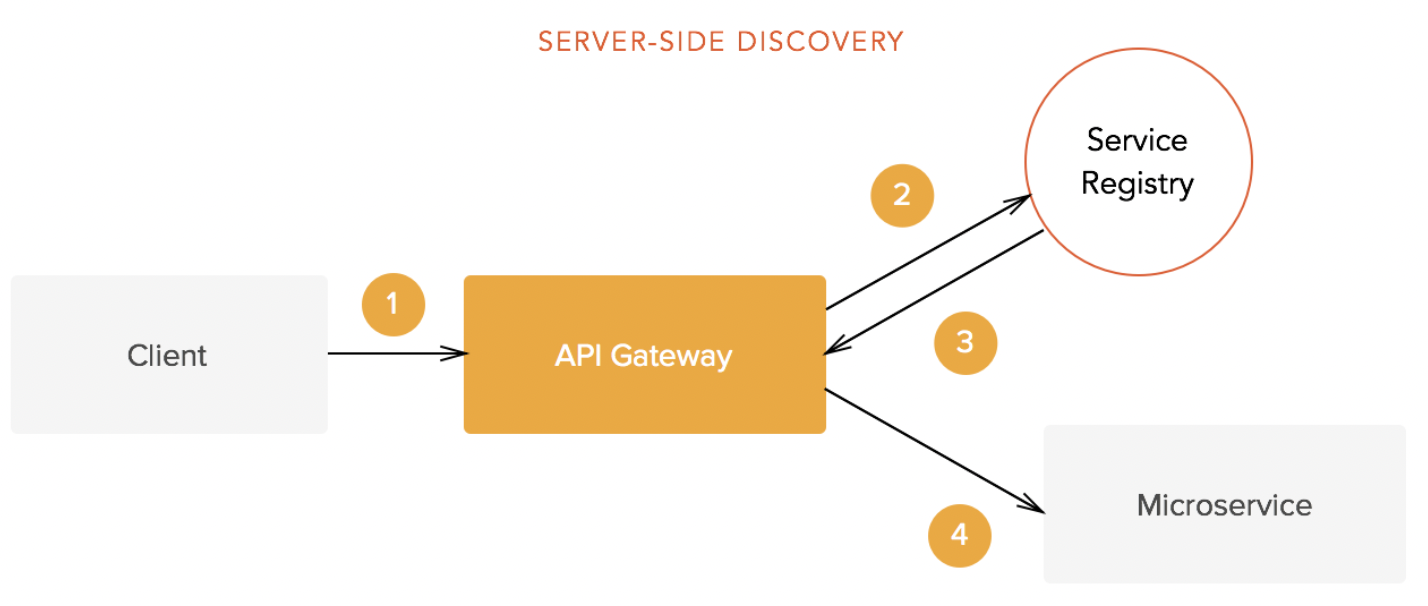
\includegraphics[width=0.7\linewidth]{./assets/images/case-studies/server-side-discovery.png}
  \caption{A simple service registry setup \cite{peyrott15}.}
  \label{fig:server-side-discovery}
\end{figure}

Fig. \ref{fig:server-side-discovery} depicts the gist of the service discovery pattern, and Fig. \ref{fig:cs01-arch} shows how a service registry is implemented in this case study using the Spring Cloud Netflix (Eureka) project \footnote{\url{https://spring.io/projects/spring-cloud-netflix}}. The server and client Maven dependencies are \code{spring-cloud-starter-netflix-eureka-server} and \code{spring-cloud-starter-netflix-eureka-client} respectively. The \code{eureka-server} service uses an \code{@EnableEurekaServer} annotation in its main application class to denote its server status (maintaining the service registry), and every other microservice uses a corresponding \code{@EnableEurekaClient} annotation (to self-register with the Eureka server on application startup). The server and sample client Configuration are shown in the following listings:

\begin{lstlisting}[caption=Snippet from Eureka server's application properties]
  eureka:
    client:
      register-with-eureka: false
      fetch-registry: false
\end{lstlisting}

The server is prevented from trying to register itself. For the sample client configuration, the Spring Boot application attempts to contact the Eureka server on \code{code.client.serviceUrl.defaultZone}, which is specified in \code{docker-compose.yml}. Eureka clients also send regular heartbeat messages to the server (set using \code{lease-renewal-interval-in-seconds}) to maintain their active status. Once the server stops receiving heartbeats below an expected threshold, it starts evicting the instances from the registry; this is known as self-preservation.

\begin{lstlisting}[caption=Snippet from a Eureka client's application properties]
  eureka:
    instance:
      lease-renewal-interval-in-seconds: 5
    client:
      register-with-eureka: true
      fetch-registry: true
      serviceUrl:
        defaultZone: http://$\dollar${EUREKA_SERVER:eureka-server}:$\dollar${EUREKA_PORT:8761}/eureka/
\end{lstlisting}

Netflix Eureka also makes a dashboard available (Fig. \ref{fig:eureka-dashboard}) at the configured port (8761), which shows the active services, system status, and other useful information about memory usage, number of CPUs, server uptime, and so on.

\begin{figure}[H]
  \centering
  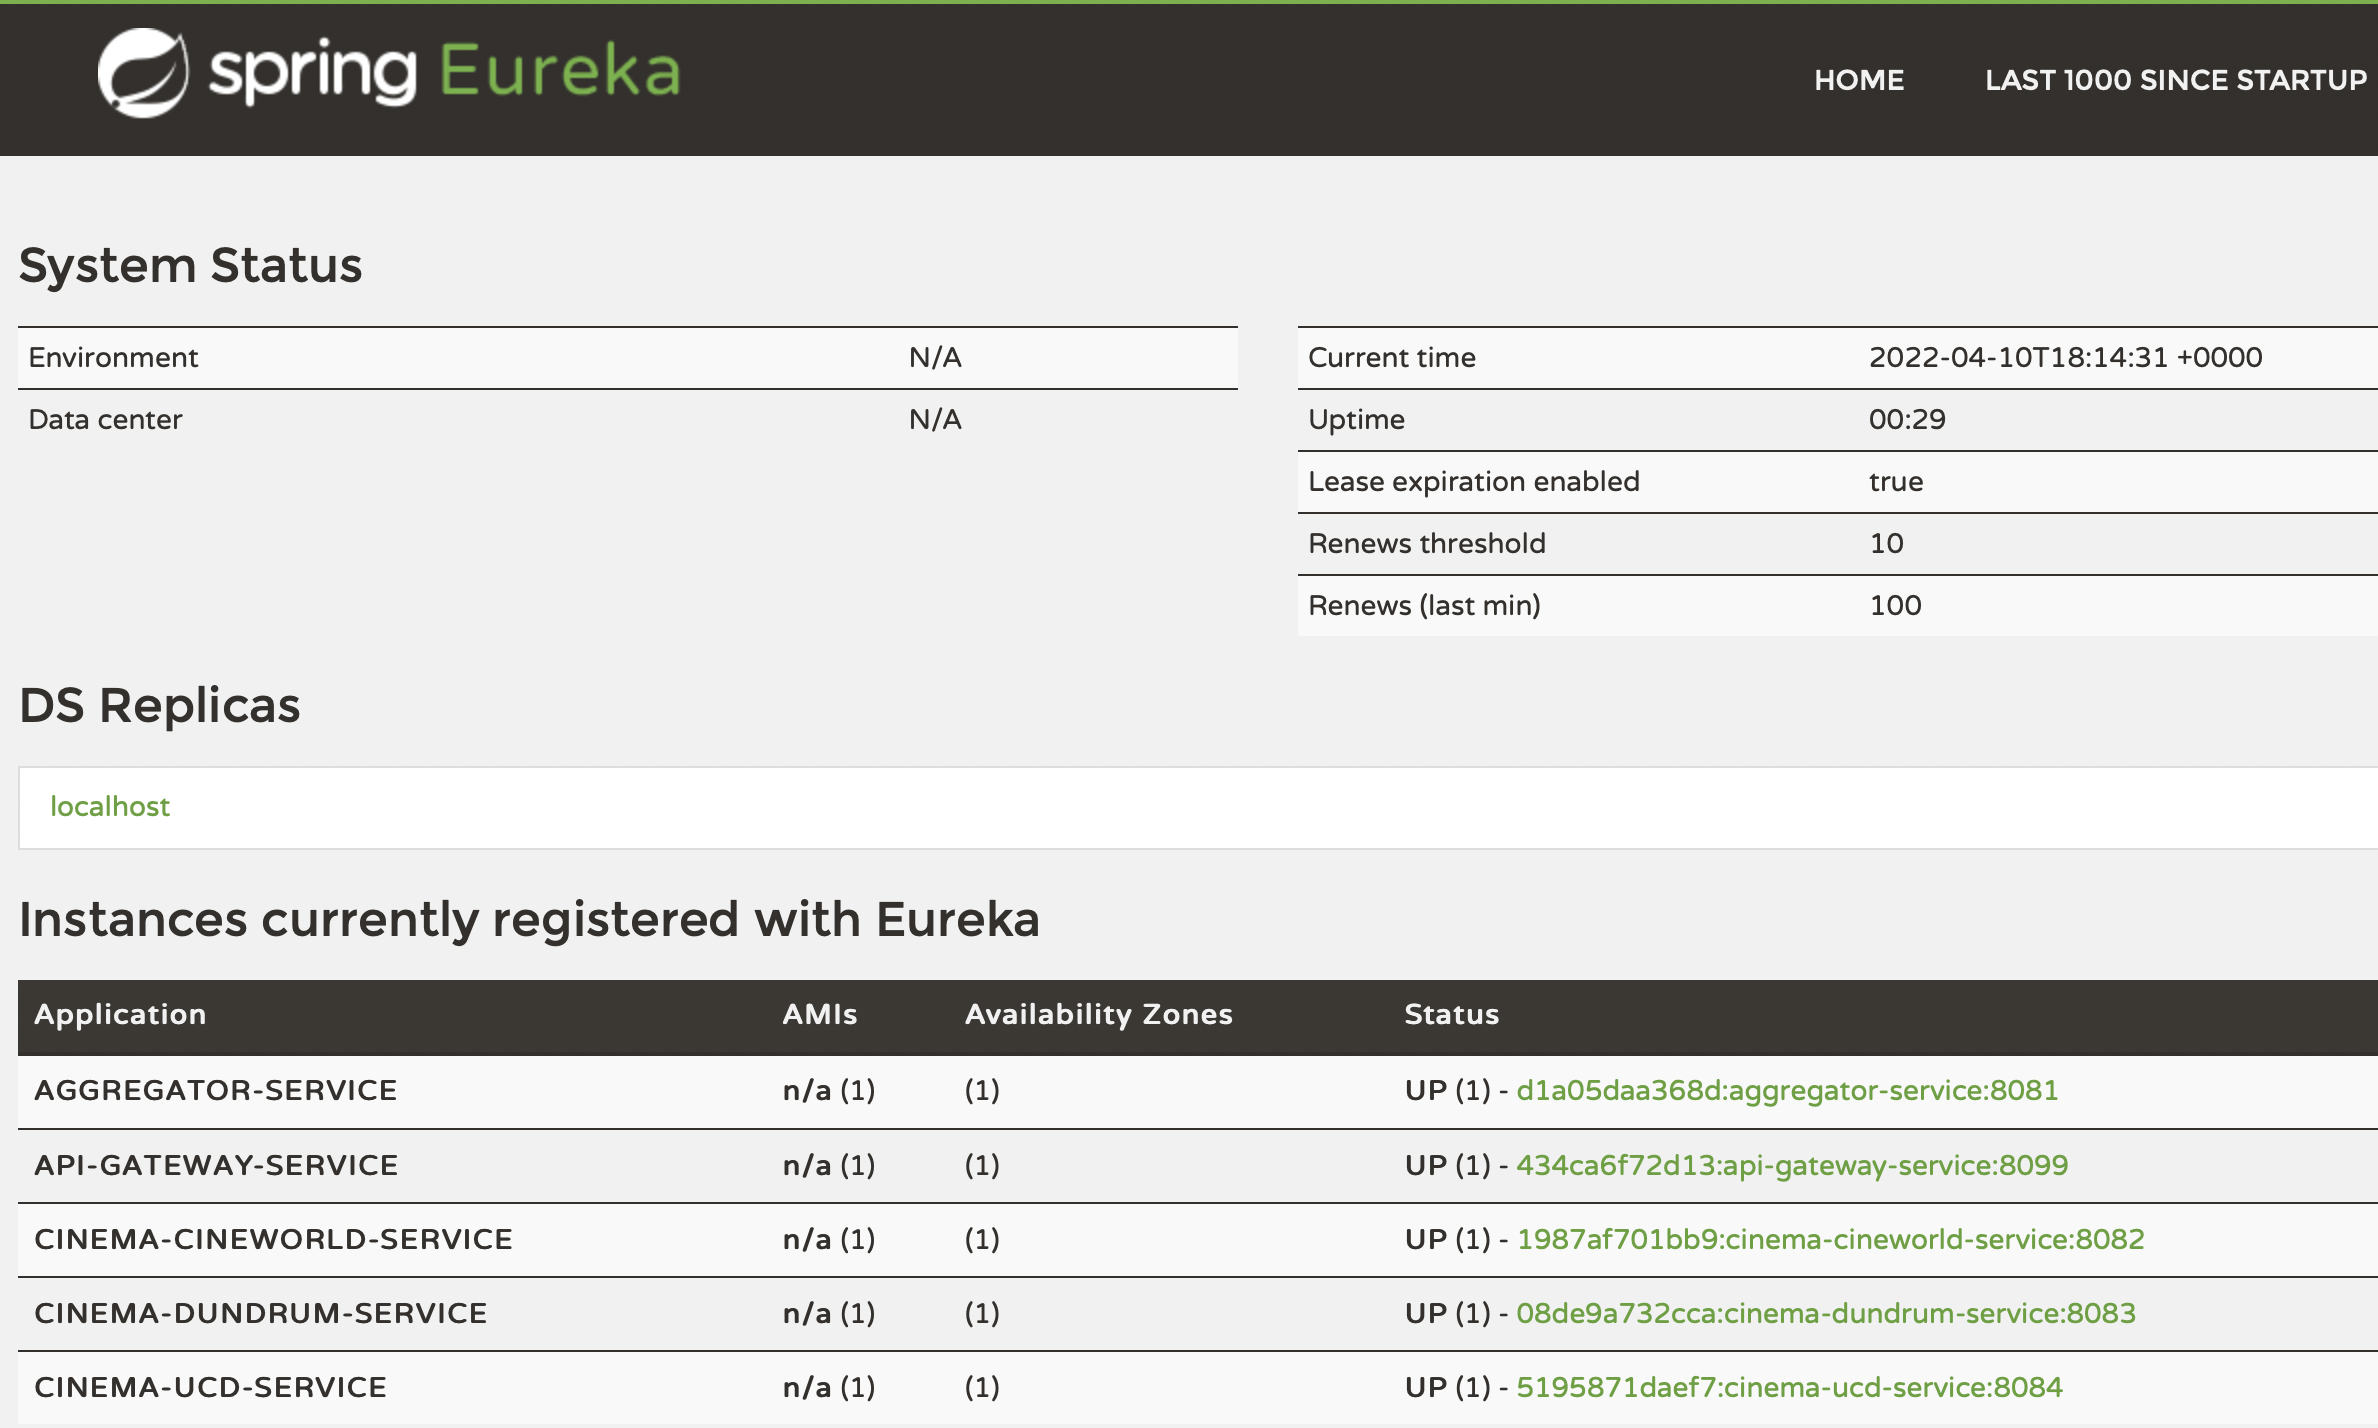
\includegraphics[width=1.0\linewidth]{./assets/images/case-studies/eureka-dashboard.png}
  \caption{Eureka dashboard}
  \label{fig:eureka-dashboard}
\end{figure}

\subsubsection{Aggregator}

The service \textit{aggregator} design pattern for microservices is useful when similar calls need to made to multiple microservices. On receiving a request from the client via an API gateway, the aggregator service dispatches the request to appropriate internal backend microservices, then combines the responses into a single structure, which is returned to the requester. The aggregator itself doesn't need to know the routing details of internal services, since it can communicate with them through the API gateway again. The performance benefit of this pattern is the reduction in communication overhead and chattiness between the client and the various internal cinema microservices.

Moreover, in this case study, the aggregator service relies on the service discovery pattern to find the registered cinema services at any given time. The code snippet from \code{aggregator-service} below illustrates how a custom discovery service function is used to fetch the addresses of all active cinemas, which the aggregator can use to send identical GET or POST requests to (received from client via the gateway). The primary advantage of this design choice is the fact that the aggregator does not need to be made aware when the number of cinema services changes, as long as the necessary registration process is completed with the Eureka server.

\begin{lstlisting}[language=Java, caption=Snippet from \code{AggregatorService.java}]
  for (String serviceUrl : discoveryService.getCinemaUrlPrefixes()) {
      String url = apiGatewayHost + serviceUrl + endpoint;
      if (httpMethod.matches("GET")) {
          results.add(restClient.getForObject(url, type));
      } else if (httpMethod.matches("POST")) {
          results.add(restClient.postForObject(url, body, type));
      }
  }
\end{lstlisting}

In the given movie ticket reservation system, the function of the aggregator is to gather the list of movie showtimes from every registered cinema, and return a compiled list to the client. It should also be noted that an alternative to an aggregator microservice is to perform response aggregation in an API gateway itself, which results in the \textit{gateway aggregation} pattern.

\subsubsection{Externalised Configuration}

Externalised configuration is a cross-cutting concerns design pattern, that is especially useful in separating changeable application properties from the business logic. Spring Boot has built-in support for processing external configuration from various sources, such as Java properties files, YAML files, environment variables, and command-line arguments. The values set by the developer for such properties are injected into Spring beans \footnote{\url{https://www.baeldung.com/spring-bean}} using the \code{@Value} annotation (among other alternatives).

Shown below are the environment variable settings for Cineworld's cinema service in the first case study's Docker Compose file.
\begin{lstlisting}[caption=Snippet from \code{docker-compose.yml}]
  cinema-cineworld-service:
    ...
    environment:
      - SERVER_PORT=8082
      - EUREKA_SERVER=eureka-server
      - DATABASE_HOST=mongodb
      - DATABASE_PORT=27017
    ...
\end{lstlisting}

Using the above environment variables, Spring Boot then sets the application properties. Externalising configuration also allows the development team to maintain all properties in one place (say the Docker Compose file) such that any required changes will only need to be made in that file, instead of searching for every occurrence of the property in the application source code.

\begin{lstlisting}[caption=Snippet from \code{cinema-cineworld-service} \code{application.yml} file]
  server:
    servlet:
      context-path: /cinema/cineworld
    port: $\dollar${SERVER_PORT}
  spring:
    application:
      name: cinema-cineworld-service
    data:
      mongodb:
        database: cinema-cineworld
        host: $\dollar${DATABASE_HOST:mongodb}:$\dollar${DATABASE_PORT:27017}
  eureka:
    ...
    client:
      ...
      serviceUrl:
        defaultZone: http://$\dollar${EUREKA_SERVER:eureka-server}:$\dollar${EUREKA_PORT:8761}/eureka/
\end{lstlisting}

\subsubsection{Database per Service}

In monolithic applications, databases are shared across services, typically in a tiered approach (involving a web tier, services tier, cache tier and data tier). However, this leads to a large central database that becomes a single performance bottleneck for all data operations, and is considered an anti-pattern when used with microservice architecture. For the microservices in our system to be truly independent, their persistent data stores must also be loosely coupled. Each service must have ownership over its domain data and logic under an autonomous lifecycle. This is achieved using the \textit{database per service} design pattern.

Database independence in microservices can possibly introduce additional concerns, as illustrated by the CAP theorem \footnote{\url{https://en.wikipedia.org/wiki/CAP_theorem}}, according to which a distributed data store can only provide two of the following: consistency, availability and partition tolerance (see also: choice between ACID and BASE transaction models \footnote{\url{https://www.geeksforgeeks.org/acid-model-vs-base-model-for-database/}}). In this project, MongoDB \footnote{\url{https://www.mongodb.com}}, a popular NoSQL database, is set up using Docker.

\begin{lstlisting}[caption=Docker Compose file snippet for MongoDB server]
  services:
    mongodb:
      image: mongo:latest
      container_name: mongodb
\end{lstlisting}

Although only a single server is used in this project (serving at the default port - 27017), every microservice is configured to use a separate database. For instance, in the code listing below, \code{spring.data.mongodb.database} is set to \code{cinema-cineworld}, which creates and uses a separate database for Cineworld service, independent from other cinemas. When dealing with services with high throughput, multiple database servers may need to be provisioned, which can be achieved with Docker service scaling or using an orchestration tool like Kubernetes. The complications of a web application's integration with a persistent data store is made trivial with the help of the Spring Data MongoDB \footnote{\url{https://spring.io/projects/spring-data-mongodb}} project.

\begin{lstlisting}[caption=Snippet from Cineworld cinema's application properties]
  spring:
    ...
    data:
      mongodb:
        database: cinema-cineworld
        host: $\dollar${DATABASE_HOST:mongodb}:$\dollar${DATABASE_PORT:27017}
\end{lstlisting}

Although all services use MongoDB in this project for the purpose of simplicity, the database per service design pattern allows every service to use a different kind of data store if the need arises, for instance, a service storing a lot of relational data could use MySQL, whereas another service storing network data might use a suitable graph database.

\subsubsection{Service Instance per Container}

As discussed in the project outline, Docker is used to containerise and deploy the microservices. The services have been built as a multi-module Maven project, each having an independent Dockerfile for deployment. Docker Compose \footnote{\url{https://docs.docker.com/compose/}} simplifies the process of defining and running multi-container Docker applications: running \code{docker-compose up} starts and runs the services defined in the Compose file, provided that each service has a valid Dockerfile.

\begin{lstlisting}[caption=Sample Docker Compose commands to start the microservices]
  docker-compose down --remove-orphans
  docker-compose build --no-cache
  docker-compose up
\end{lstlisting}

The wide range of benefits to containerising microservices make Docker the industry leading tool for service deployment. Developers are able to choose any suitable programming language and framework (including different versions), since Docker provides isolated environments with all required dependencies. The \textit{service instance per container} design pattern allows each microservice to be packaged as a Docker container image, permitting the deployment of multiple instances of the microservice as separate containers if required.

There are far reaching performance benefits of this pattern, including service reproducibility, independent deployment and scaling, hardware resource (CPU/memory) constraining capabilities, service instance monitoring, reliability and fault tolerance. Most importantly, Docker containers are much faster than traditional virtual machines (VMs) thanks to lightweight architecture (sharing the host OS kernel instead of requiring a complete OS or hypervisor). In large scale projects, container orchestration tools such as Kubernetes \footnote{\url{https://kubernetes.io}}, Marathon (Mesos) \footnote{\url{https://mesosphere.github.io/marathon/}}, Amazon ECS \footnote{\url{https://aws.amazon.com/ecs/}} and EKS \footnote{\url{https://aws.amazon.com/eks/}} are widely used to automate the operational effort required to manage containerised microservices, which is key for well-run DevOps.

The three cinema microservices have identical Dockerfiles, as shown below. Each of them use a JDK 11 base image, copy the compiled JAR file into the container, then run it after a 5 second wait. Using Docker Compose, each service's Dockerfile is used to start the application.

\begin{lstlisting}[caption=Dockerfile for cinema services]
  FROM openjdk:11-jre-slim
  COPY target/cinema*.jar /cinema.jar
  CMD sleep 5 && java -jar /cinema.jar
\end{lstlisting}


\subsection{Evaluation}

In order to evaluate the first case study, the aforementioned plan involving performance modelling, manual API testing and JMeter load testing is followed.

\subsubsection{Performance Modelling}

Fig. \ref{fig:cs01-sequence} shows a sequence diagram for a scenario where the client wishes to fetch the list of movie showtimes from all active cinema microservices, and view the aggregated results. The digram components follow the specifications from OMG (2011) \cite{omg11}, showing a series of \textit{objects} (e.g. Client, Aggregator, Cinemas) with vertical \textit{lifelines} (downward flow of time). Opaque rectangles on top of lifelines are \textit{activation boxes} (i.e. method-invocation boxes) which indicate an object handling/processing a message.

\begin{figure}[H]
  \centering
  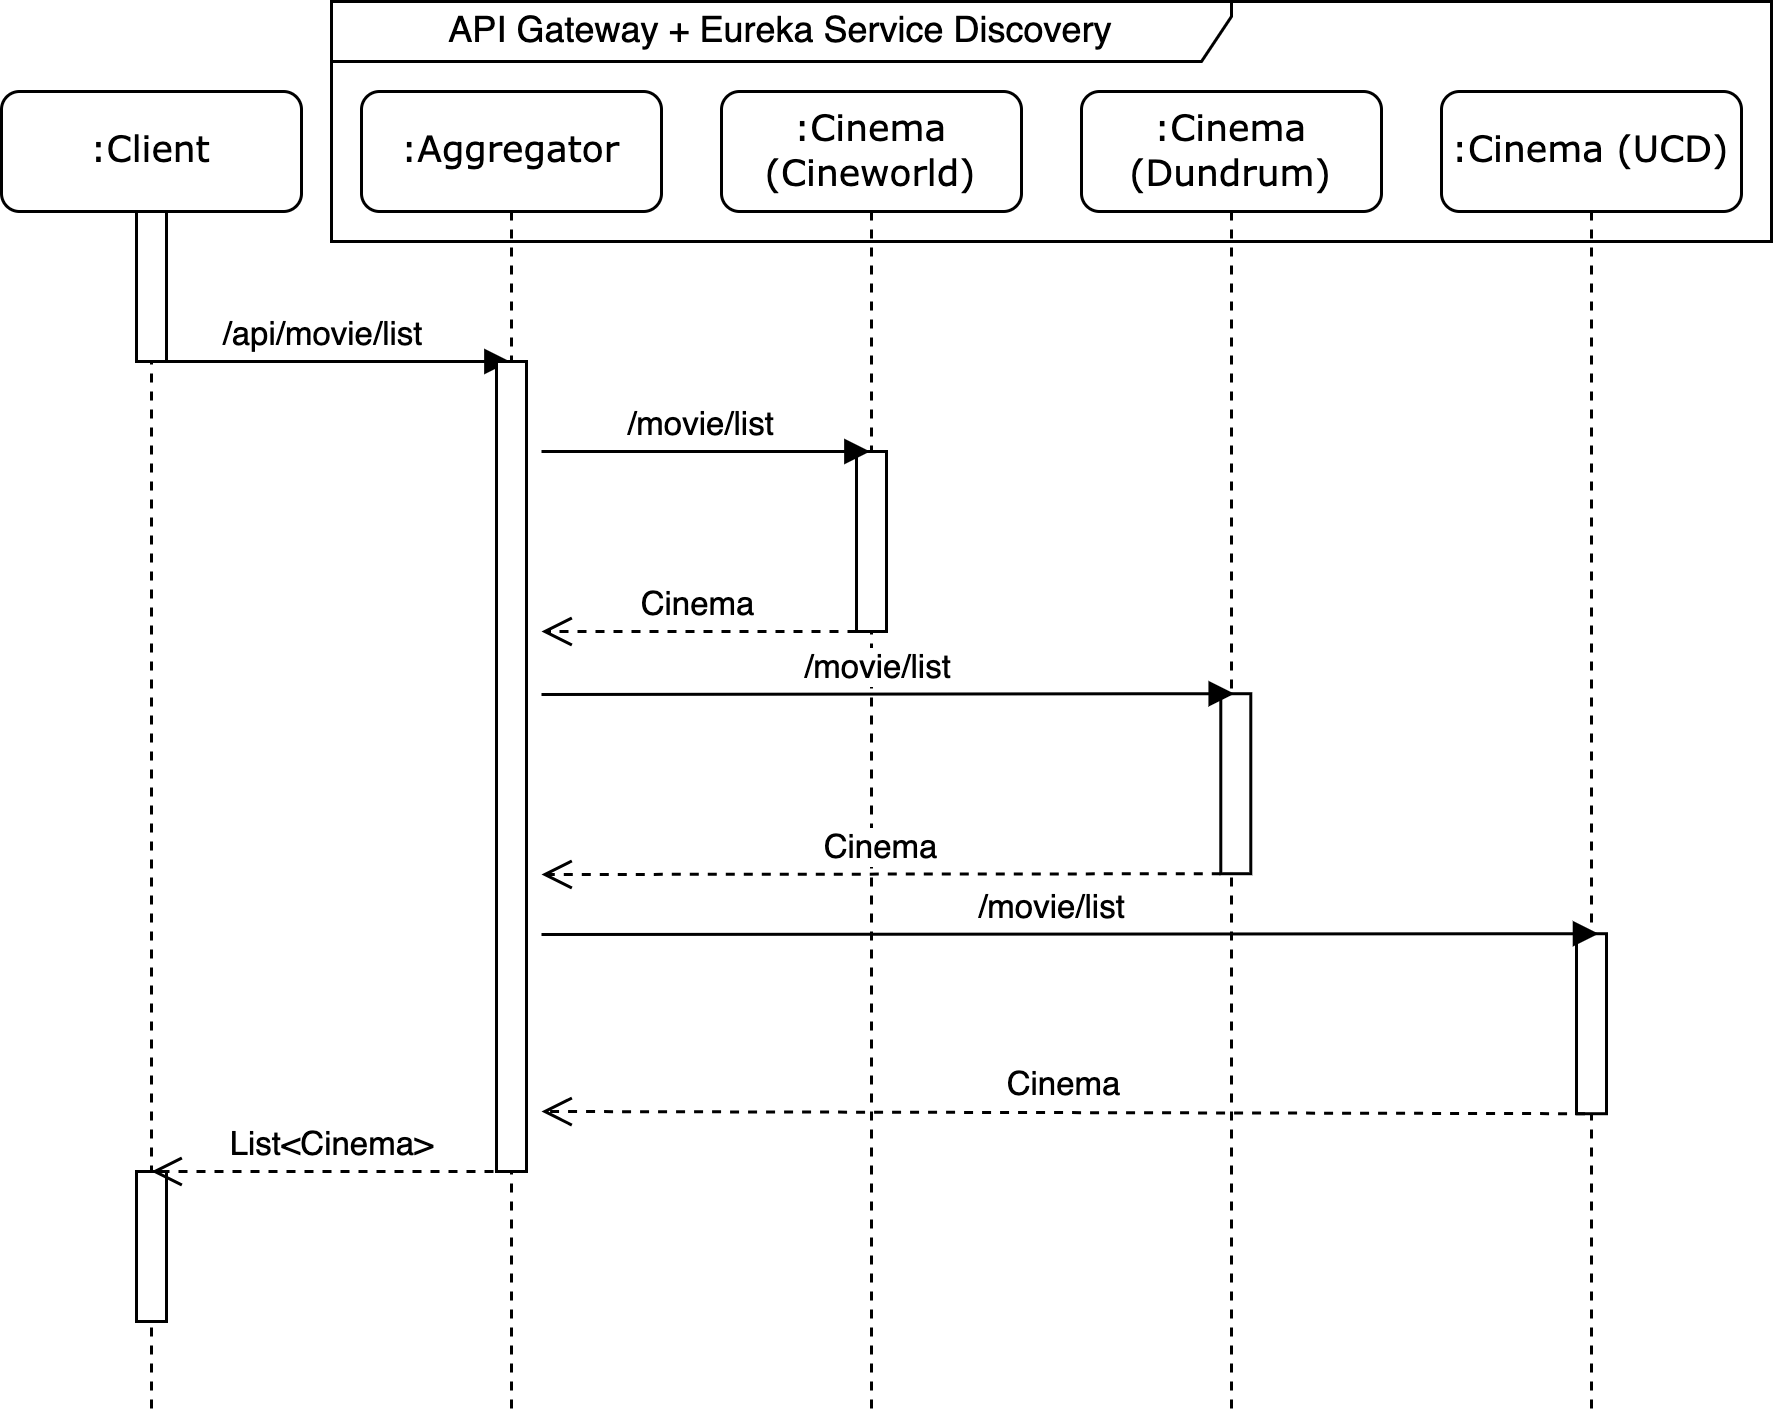
\includegraphics[width=0.75\linewidth]{./assets/diagrams/cs01-sequence.png}
  \caption{UML sequence diagram for listing movies from all cinemas (case study 1).}
  \label{fig:cs01-sequence}
\end{figure}

Sequence of steps:
\begin{itemize}
  \item Client calls the API endpoint \code{/api/movie/list} exposed by the Aggregator service, via the API gateway and Eureka service discovery. All synchronous calls are represented by closed arrow heads with solid lines.
  \item When received (dashed lines) by the Aggregator, it requests each active Cinema service (again via the gateway, discovering the ports using Eureka), for their respective list of movie showtimes.
  \item Each service responds with a \code{Cinema} object, containing a unique identifier, cinema name, and list of movies (including showtimes).
  \item The Aggregator then combines all \code{Cinema} objects into a list, to return to the Client.
  \item Since this entire flow is synchronous, the connection between the Client and Aggregator remains open while the latter contacts all cinemas.
\end{itemize}

From the sequence diagram, one can infer that the API gateway (and possibly the aggregator) service can turn into potential performance bottlenecks if appropriate preventive measures are not taken under heavy load, especially since all the inter-service communication is synchronous and blocking. Similar modelling can also be done for other use cases, such as making a reservation, or listing reservations at a given cinema.

\subsubsection{Manual API Testing}

Using VS Code, the time taken by the application to process a given HTTP request (stored under \code{src/main/resources/http/} in \code{api-gateway-service}) was measured. All calls were made to the client-facing API gateway on port 8099, which internal microservices also use to communicate with each other. The following endpoints were tested to demonstrate the functionality of the web application:

\begin{itemize}
  \item \code{/api/movie/list} (Fig. \ref{fig:cs01-manual-1}): As specified in the API gateway routing configurations, all requests to \code{/api} are forwarded to the Aggregator service using a logical address. Actual network locations are maintained only by the Eureka service registry, where all services must register on startup. A GET request to the \code{/api/movie/list} endpoint returns the list of movie showtimes (HTTP status 200 OK) from all active cinema services in 153 milliseconds (ms).

  \item \code{/cinema/cineworld/reservation/make} (Fig. \ref{fig:cs01-manual-2}): A sample ticket reservation can be made at Cineworld by directing the request only to the appropriate service, using a POST request to \code{/cinema/cineworld/reservation/make}. The body of the request includes booking details such as the client name and email, movie ID, date, showtime, number of tickets, ticket type/category and total amount paid. In a production system, these details would be provided by the frontend, after the client enters information on a website. An HTTP status 201 Created response implies that the reservation was successfully stored in the cinema database, with the server returning the new reservation in 152 ms.

  \item \code{/cinema/cineworld/reservation/list} (Fig. \ref{fig:cs01-manual-3}): To ensure that the previous reservation at Cineworld was successful, one can list all the reservations at Cineworld. In a production system, such an endpoint would be privileged and restricted to admin users, so that any external client doesn't get access to other clients' booking details. A 200 OK response in 45 ms returns a list of reservations, containing a single entry for Jane Doe's booking made earlier.

  \item \code{/cinema/cineworld/reservation/delay/4} (Fig. \ref{fig:cs01-manual-4}): To illustrate a working circuit breaker implementation, a simple \code{/delay/4} endpoint for Cineworld can be invoked, which simply sleeps for 4 seconds. To prevent unresponsive services, the circuit breaker in the API gateway has been configured to time out after 3 seconds, and display a fallback message (HTTP code 500 Internal Server Error) containing the service name where the timeout occurred.
\end{itemize}


\subsubsection{Performance Testing}

Finally, using CLI mode on Apache JMeter, the microservices can be load tested. Two test plans (A and B) have been designed: to fetch the list of movie showtimes from all cinemas, and then to make a ticket reservation at Cineworld. For both tests, the number of threads (users) is varied from 10 to 100 in intervals of 10, with a ramp-up period of 1 second, i.e. the time taken by JMeter to get all threads up and running. Importantly, all load testing is performed over 1000 iterations to improve reliability of measurements.

\begin{figure}[H]
  \centering
  \subfigure[]{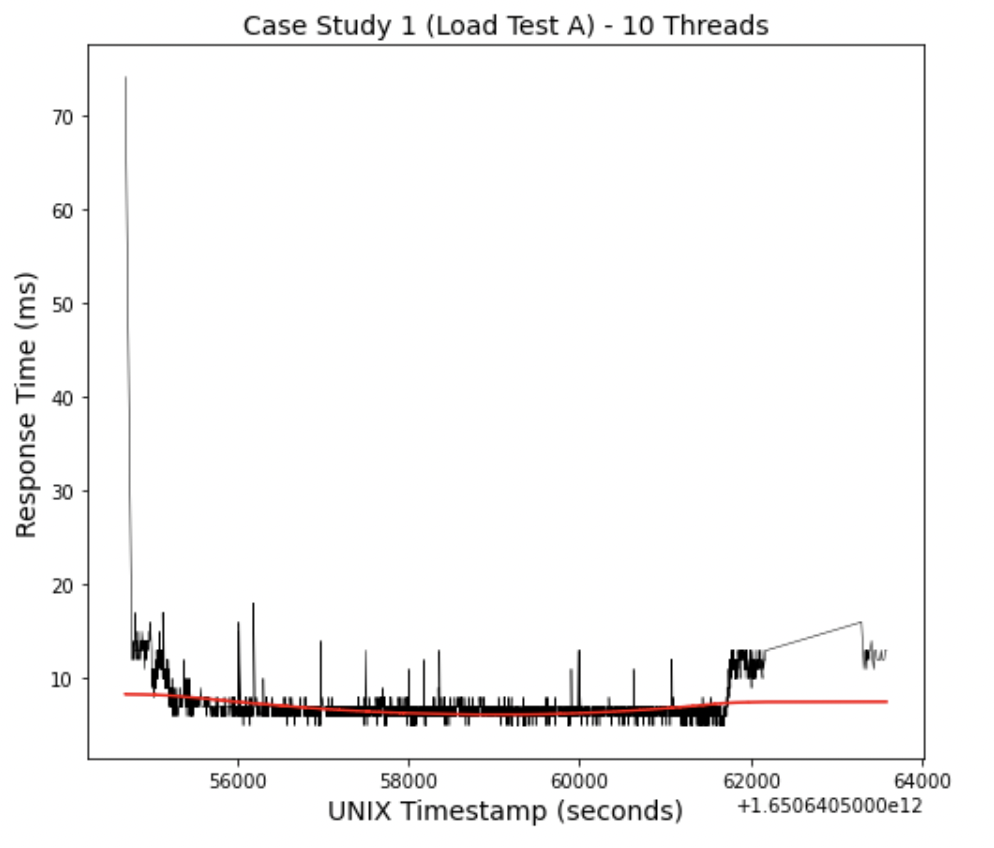
\includegraphics[width=0.45\linewidth]{./assets/images/case-studies/cs01-lta-1.png}}
  \subfigure[]{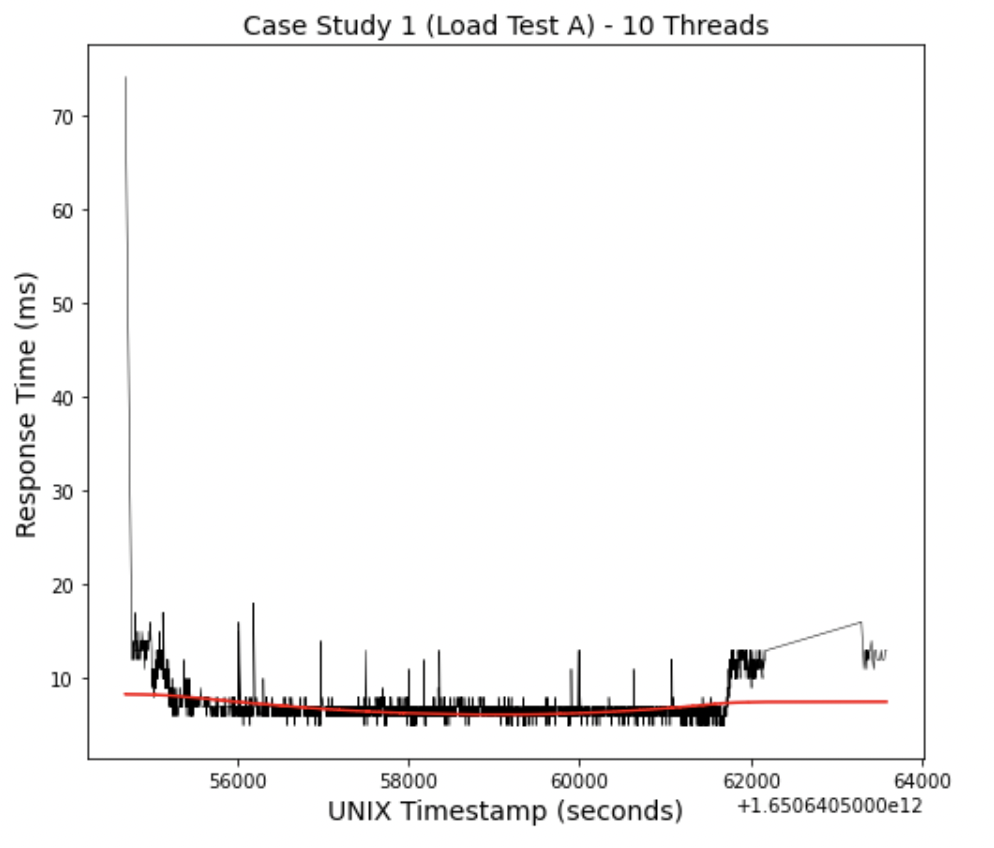
\includegraphics[width=0.5\linewidth]{./assets/images/case-studies/cs01-lta-2.png}}
  \caption{Load test A response times using (a) 10 threads and (b) 100 threads.}
  \label{fig:cs01-lta-12}
\end{figure}

Load test A is focussed on the \code{/api/movie/list} endpoint, with the call to the aggregator service (via API gateway) returning the full list of movie showtimes from Cineworld, Dundrum and UCD cinemas. Fig. \ref{fig:cs01-lta-12} shows the response times measured at the two load extremities - 10 threads and 100 threads. Since response time measurements are known to be noisy, a Savitzky-Golay filter is used for data smoothing (plotted in red). The filter uses convolution, by applying the linear least squares method to fit successive subsets (chosen size = 10000) of adjacent data points with a low degree polynomial (chosen = 2). The results show that at a low workload of 10 threads, the response time is more or less constant at under 10 milliseconds (ms). There is a noticeable initial spike (70 ms +), likely due to the time taken to establish the database connection and populate the cache (cold start). The load is increased in intervals of 10 threads, up to the heavy load scenario of 100 threads. In that situation, the recorded response times jumped from 30-50 ms to about 100 ms (noticeable in the plot between timestamp 270000 and 280000). The variation in response time appears to increase significantly when using 100 threads, suggesting a need for system scaling to handle heavier workloads without performance degradation.

\begin{figure}[H]
  \centering
  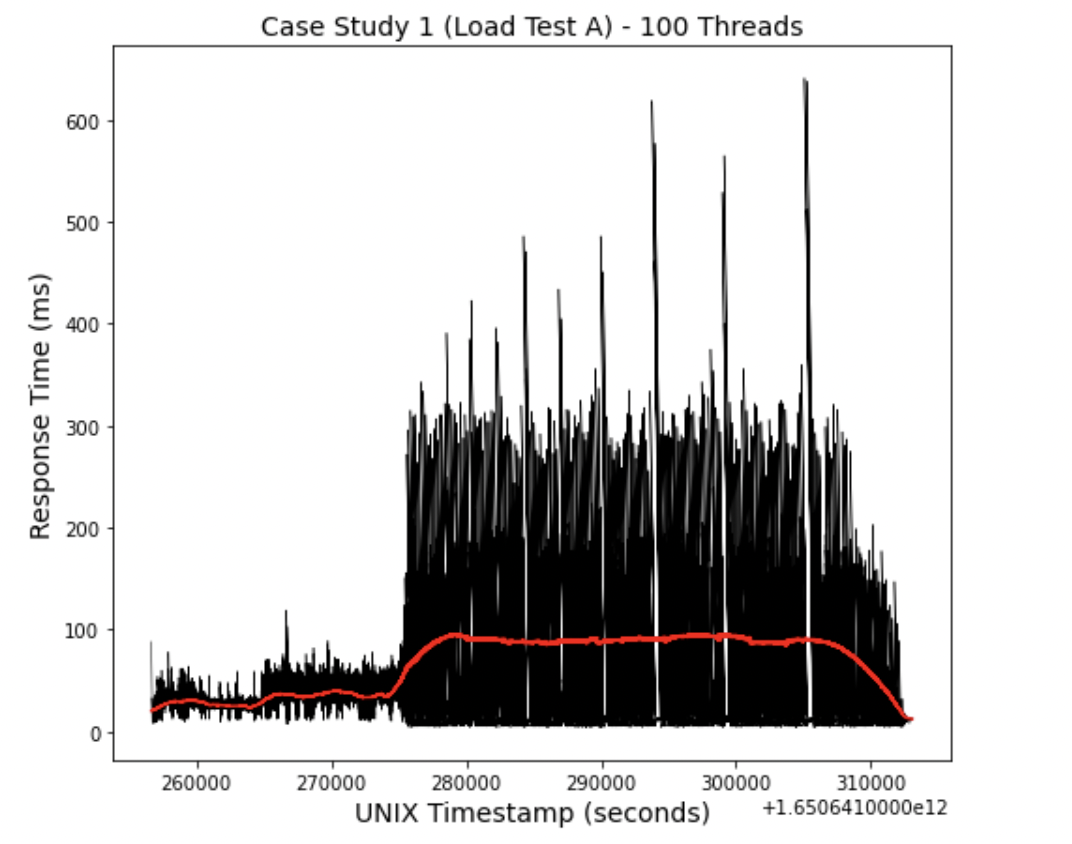
\includegraphics[width=0.6\linewidth]{./assets/images/case-studies/cs01-lta-3.png}
  \caption{Count of 200 and 500 HTTP response codes during load test A at different load levels.}
  \label{fig:cs01-lta-3}
\end{figure}

Fig. \ref{fig:cs01-lta-3} shows the response codes observed during load test A, 200 implying success and 500 signifying a server error. The circuit breaker timeout pattern employed in this case study prevents unresponsive server behaviour at heavy workloads, with fast failures reflected by the increase in proportion of errors (16 to 20\%) at load points such as 90 or 100 threads. This is preferable to the server taking 3 plus seconds to respond to client queries. However, steps must be taken to minimise the error probability - with the recommended approach being an increase in service capacity (horizontal or vertical scaling as appropriate) to handle heavier load.

\begin{figure}[H]
  \centering
  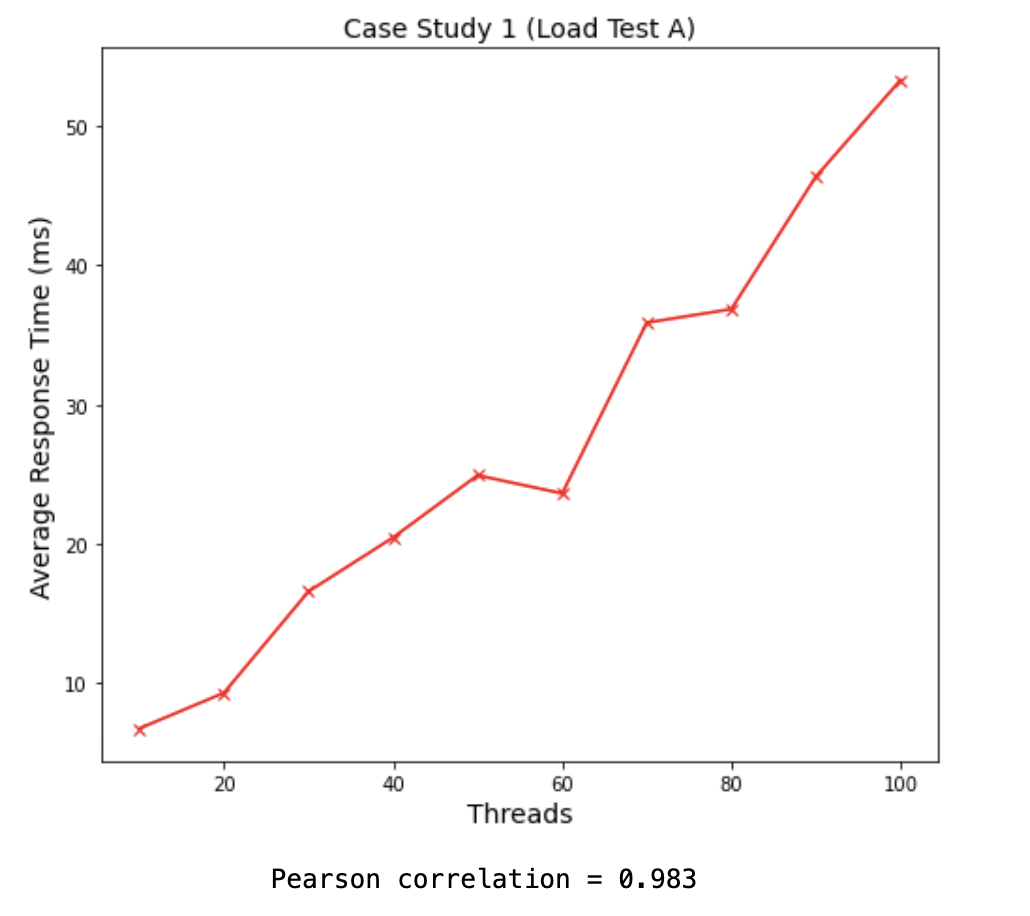
\includegraphics[width=0.55\linewidth]{./assets/images/case-studies/cs01-lta-4.png}
  \caption{Average response time vs number of threads in load test A.}
  \label{fig:cs01-lta-4}
\end{figure}

One of the primary aims of load testing is to demonstrate the system resource usage being proportional to the applied load, which is a precondition for scalability. This is well illustrated by Fig. \ref{fig:cs01-lta-4}, with a strong positive Pearson correlation of 0.983 between average response time and the number of threads (load).

For load test B, a similar strategy as above was applied to check the ticket reservation functionality of the application. The API endpoint \code{/cinema/cineworld/reservation/make} directly contacts the Cineworld service via the API gateway. Due to the reduced inter-service communication, the response times measured at both load extremities - 10 threads and 100 threads are more or less constant at about 3 ms and 10 ms respectively. As expected, making a reservation at a single cinema is considerably quicker than aggregating movie showtimes from all services. The listing below shows the ticket booking details used as the POST request body - identical to the payload used for manual API testing.

\begin{lstlisting}[caption=Dummy payload for load test B POST request]
  {
    "clientName": "Jane Doe",
    "clientEmail": "jane.doe@ucd.ie",
    "movieId": "CNW001",
    "date": "2022-04-15",
    "showTime": "18:00",
    "tickets": 2,
    "ticketType": "Gold",
    "amount": 30.00
  }
\end{lstlisting}


\begin{figure}[H]
  \centering
  \subfigure[]{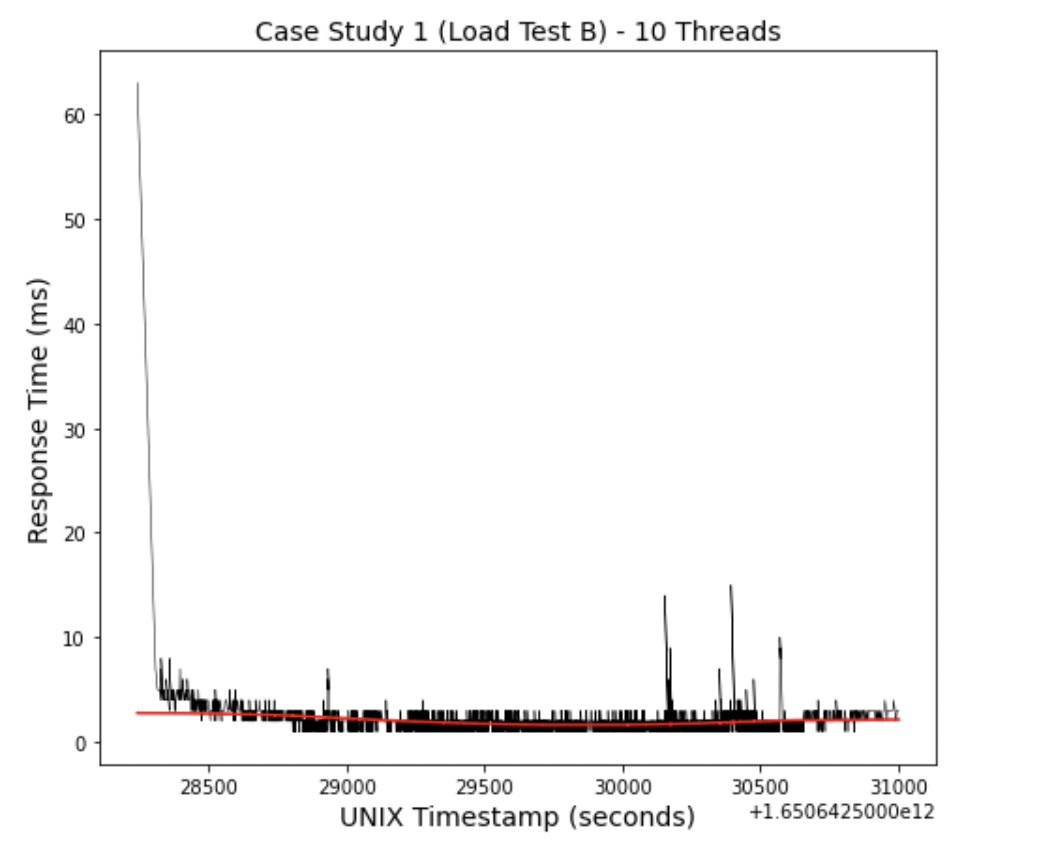
\includegraphics[width=0.45\linewidth]{./assets/images/case-studies/cs01-ltb-1.png}}
  \subfigure[]{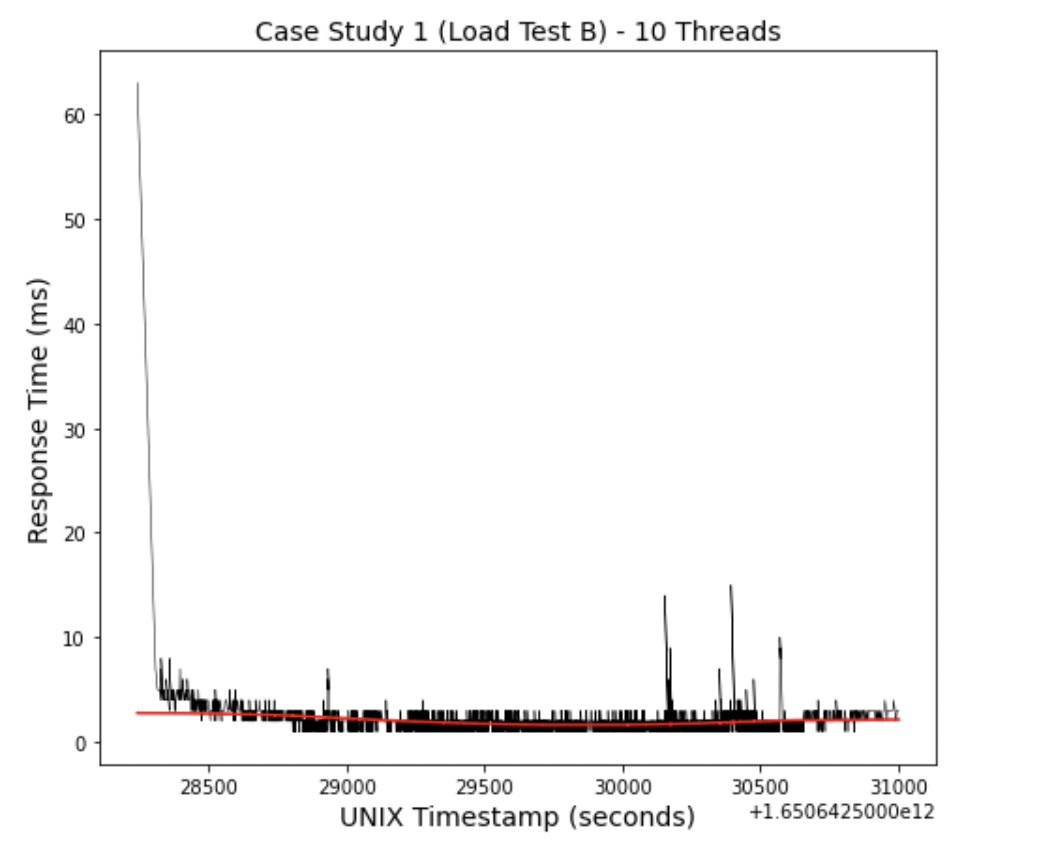
\includegraphics[width=0.45\linewidth]{./assets/images/case-studies/cs01-ltb-2.png}}
  \caption{Load test B response times using (a) 10 threads and (b) 100 threads.}
  \label{fig:cs01-ltb-12}
\end{figure}

Fig. \ref{fig:cs01-ltb-3} showing a 100\% success rate (all 201 Created HTTP response codes) at all load levels reaffirms the fact that relatively low response times for reservation requests allows the system to handle a load even greater than 100 threads per second before collapsing and requiring a scale-up.


\begin{figure}[H]
  \centering
  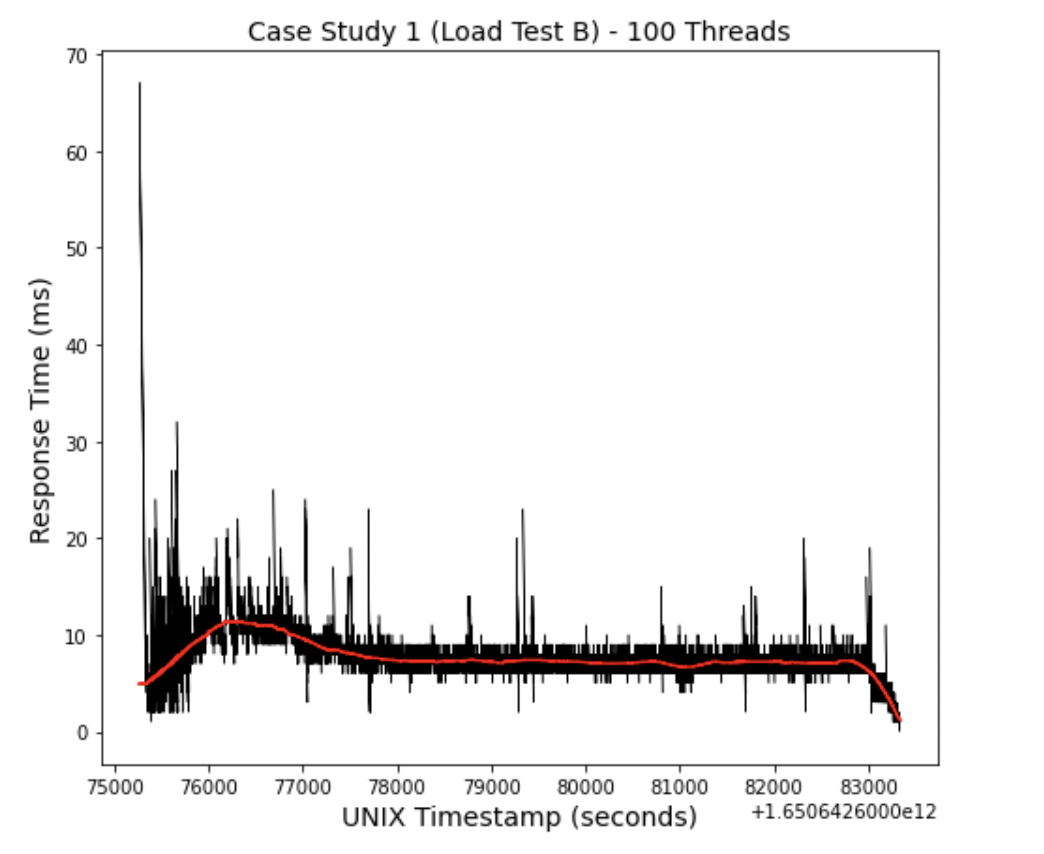
\includegraphics[width=0.6\linewidth]{./assets/images/case-studies/cs01-ltb-3.png}
  \caption{Count of HTTP response codes during load test B at different load levels.}
  \label{fig:cs01-ltb-3}
\end{figure}

As seen before in load test A, the linearity of resource consumption with respect to system load in test B is confirmed by a Pearson correlation score of 0.985. The straight line plot in Fig. \ref{fig:cs01-ltb-4} shows a proportional increase in mean response time with load increasing gradually from 10 to 100 threads.

\begin{figure}[H]
  \centering
  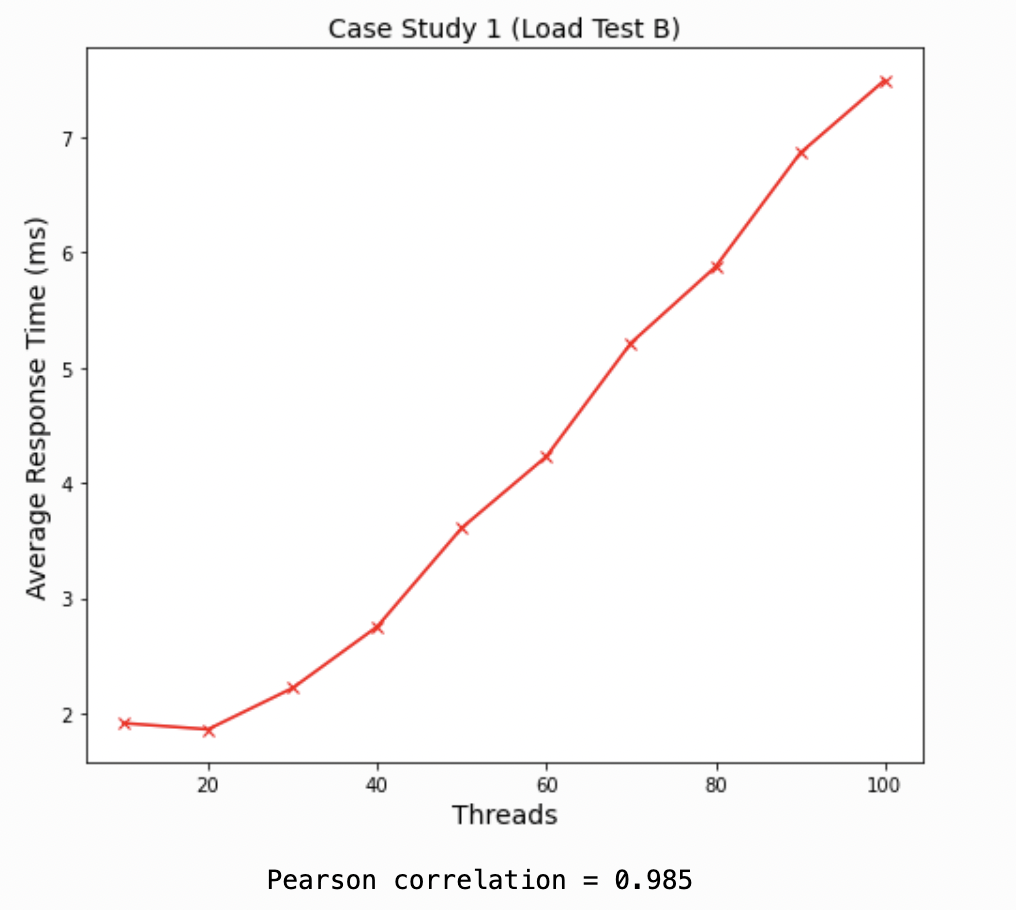
\includegraphics[width=0.55\linewidth]{./assets/images/case-studies/cs01-ltb-4.png}
  \caption{Average response time vs number of threads in load test B.}
  \label{fig:cs01-ltb-4}
\end{figure}